% Advanced Robotics Project (NBVHR1HBNF) -- Week 1: Classical Robotics
% Obuda University, Antal Bejczy Center for Intelligent Robotics
% Uses the ABC-iRobotics BARK beamer template (bark169).
% Required next to this file: beamerthemebark169.sty, img/, src/

\documentclass[aspectratio=169]{beamer}
\usepackage[english]{babel}
\usetheme{bark169}

\usepackage{tikz}
\usetikzlibrary{arrows.meta,positioning,shapes.geometric,calc}
\usepackage{booktabs}
\usepackage{animate}  % animations play in Adobe Acrobat Reader; other viewers show the poster frame

\title[Classical Robotics]{Advanced Robotics Project\\Week 1: Classical Robotics}
\date{11 September 2026 \\ Budapest}
\author[iRob]{Panna Zsoldos, Tam\'as Piricz \\ \texttt{irob.uni-obuda.hu}}

% "In one sentence" box at the bottom of concept slides
\newcommand{\takeaway}[1]{\vspace{2mm}\begin{beamercolorbox}[rounded=true,sep=4pt,wd=\textwidth]{block body}\footnotesize\textbf{In one sentence:} #1\end{beamercolorbox}}
% Vocabulary recap slide
\newcommand{\wordsframe}[1]{\begin{frame}{Words to keep}\begin{center}\Large #1\end{center}\end{frame}}
% One labelled photo in a 3-column grid (robot types slide)
\newcommand{\robotcell}[2]{\begin{minipage}[t]{0.31\textwidth}\centering\parbox[c][2.45cm][c]{\textwidth}{\centering\includegraphics[height=2.35cm,width=\textwidth,keepaspectratio]{#1}}\\[0.8mm]#2\end{minipage}}

\begin{document}

% ===================== 0. INTRO =====================
\begin{frame}
	\titlepage
\end{frame}

{\setbeamertemplate{background}{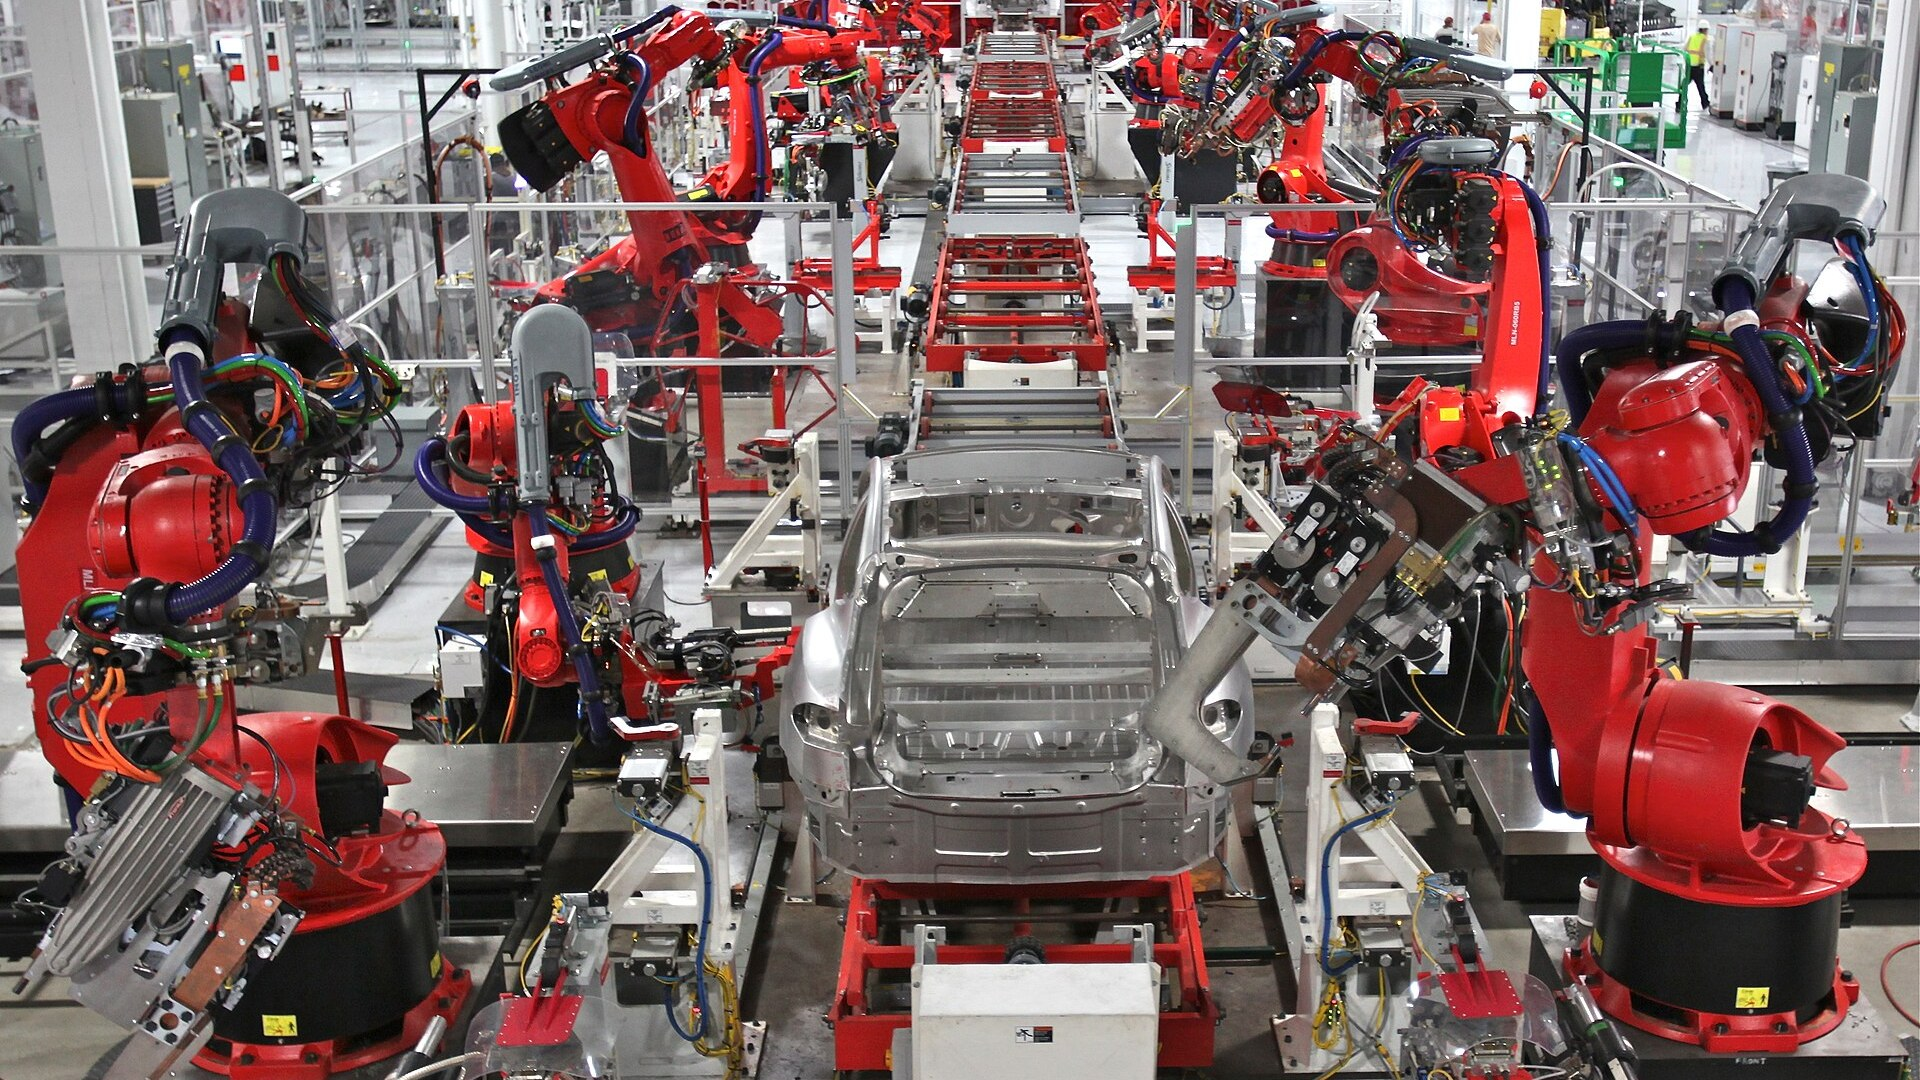
\includegraphics[width=\paperwidth,height=\paperheight]{img/web/opener_kuka_line.jpg}}
\begin{frame}[plain,b]
	\hfill\colorbox{black!60}{\tiny\color{white}Photo: Steve Jurvetson, CC BY 2.0, cropped}
\end{frame}}

\begin{frame}{Why this course exists}
	\begin{center}
		\resizebox{\textwidth}{!}{%
		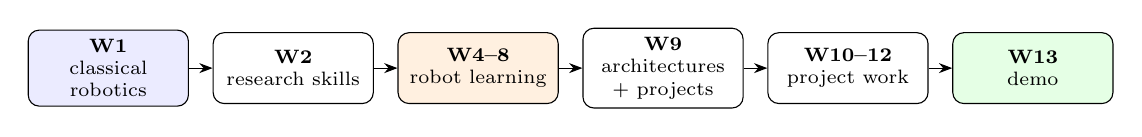
\begin{tikzpicture}[node distance=3mm, every node/.style={font=\scriptsize},
			box/.style={draw, rounded corners, minimum height=9mm, text width=18mm, align=center}]
			\node[box, fill=blue!8] (w1) {\textbf{W1}\\classical robotics};
			\node[box, right=of w1] (w2) {\textbf{W2}\\research skills};
			\node[box, right=of w2, fill=orange!12] (w468) {\textbf{W4--8}\\robot learning};
			\node[box, right=of w468] (w9) {\textbf{W9}\\architectures\\+ projects};
			\node[box, right=of w9] (proj) {\textbf{W10--12}\\project work};
			\node[box, right=of proj, fill=green!10] (demo) {\textbf{W13}\\demo};
			\draw[-{Stealth}] (w1) -- (w2); \draw[-{Stealth}] (w2) -- (w468);
			\draw[-{Stealth}] (w468) -- (w9); \draw[-{Stealth}] (w9) -- (proj);
			\draw[-{Stealth}] (proj) -- (demo);
		\end{tikzpicture}}
	\end{center}
	\vspace{3mm}
	\begin{itemize}
		\item Today: how robots were made to work \textbf{before} machine learning. The vocabulary and the building blocks.
		\item From week 4: the same problems, solved by \textbf{learning from data}.
		\item This is a practical course. You will build things with different tools, every week.
	\end{itemize}
\end{frame}

\begin{frame}{The semester at a glance}
	\begin{center}\scriptsize
	\begin{tabular}{cllc}
		\toprule
		\textbf{Week} & \textbf{Date} & \textbf{Topic} & \textbf{Deadline} \\
		\midrule
		1  & 11 Sep & Classical robotics. Semester requirements & \textbf{H1 out} \\
		2  & 18 Sep & Literature research and scientific skills & \\
		3  & 25 Sep & \textit{no class, rectorial break} & \\
		4  & 02 Oct & Supervised and unsupervised learning & \textbf{H1 due} \\
		5  & 09 Oct & \textit{no class} & \\
		6  & 16 Oct & Reinforcement, imitation, self-supervised learning & \textbf{H2 out} \\
		7  & 23 Oct & \textit{no class, public holiday} & \\
		8  & 30 Oct & Representations in robotics & \\
		9  & 06 Nov & Modern robot architectures. Project topics & \textbf{H2 due, projects out} \\
		10 & 13 Nov & Consultation 1 & \\
		11 & 20 Nov & Consultation 2 & \\
		12 & 27 Nov & Consultation 3 & \\
		13 & 04 Dec & \textbf{Project presentations} & \textbf{project due} \\
		14 & 11 Dec & Retake presentations & \\
		\bottomrule
	\end{tabular}
	\end{center}
	\vspace{1mm}
	\footnotesize Six contact classes, Fridays from 09:00. Weeks 1, 2 and 9 with Panna; weeks 4, 6 and 8 with Tam\'as.
\end{frame}

\begin{frame}{What you have to do to pass}
	\begin{center}\small
	\begin{tabular}{p{0.26\textwidth}p{0.36\textwidth}p{0.26\textwidth}}
		\toprule
		\textbf{What} & \textbf{Requirement} & \textbf{When} \\
		\midrule
		Attendance & at least \textbf{70\%} of contact classes, register taken every time & weeks 1, 2, 4, 6, 8, 9 \\
		Homework 1 & individual, submitted work & out today, due 2 Oct \\
		Homework 2 & individual, submitted work & out 16 Oct, due 6 Nov \\[1mm]
		Semester project & in teams, one of four topics & topics 6 Nov, demo 4 Dec \\
		\bottomrule
	\end{tabular}
	\end{center}
	\vspace{2mm}
	\begin{itemize}\footnotesize
		\item Your \textbf{homework points} decide the order in which teams choose their project topic.
		\item The project is graded on three things: the \textbf{documentation} (can someone else reproduce it?), a \textbf{short video}, and the \textbf{live demo}.
		\item Missed the presentation? One retake in week 14, or in the first week of the exam period by arrangement.
	\end{itemize}
\end{frame}

\begin{frame}{Grades, and one thing that is not on the list}
	\begin{columns}[T]
		\begin{column}{0.36\textwidth}
			\centering \small
			\begin{tabular}{ll}
				\toprule
				86--100\,\% & excellent (5) \\
				71--85\,\% & good (4) \\
				56--70\,\% & satisfactory (3) \\
				41--55\,\% & pass (2) \\
				0--40\,\% & fail (1) \\
				\bottomrule
			\end{tabular}
		\end{column}
		\begin{column}{0.6\textwidth}
			\begin{itemize}\footnotesize
				\item There is \textbf{no exam} and no written test. Everything is coursework.
				\item Slides and notebooks go to Moodle.
				\item \textbf{Bring your own laptop} to every class. Everything we use runs in a browser and is free.
				\item Project topics are chosen so that good results can be \textbf{written up as a paper}. That is on offer, not required.
			\end{itemize}
		\end{column}
	\end{columns}
\end{frame}

\begin{frame}{The four project topics}
	\begin{enumerate}
		\item \textbf{Object manipulation with a Shadow hand}, using Gaussian-splatting models through learning.
		\item \textbf{Humanoid torso}: building and bringing it up.
		\item \textbf{Biped robot}: building and bringing it up.
		\item \textbf{Surgical robotics} (da Vinci platform), \emph{to be confirmed}.
	\end{enumerate}
	\vspace{4mm}
	Details and team formation in week 9, after H2. Teams pick in the order of their homework points.
\end{frame}

\begin{frame}{Today}
	\begin{tabular}{ll}
		\toprule
		09:05 & A robot in the room; rules of the semester \\
		09:20 & What is a robot; types and classification \\
		09:35 & \textbf{Lab tour}: classify the real ones \\
		09:55 & Where is the hand? Frames, forward and inverse kinematics \; \textit{(Notebook 1)} \\
		10:35 & Break \\
		10:50 & How a robot sees: sensors, SLAM \\
		11:02 & How a robot drives: a warehouse robot \; \textit{(Notebook 2)} \\
		11:32 & How behaviour is built; the industry; homework \\
		\bottomrule
	\end{tabular}
\end{frame}

% ===================== 1. WHAT IS A ROBOT =====================
\section{Robot types}

\begin{frame}{One definition that survives}
	\begin{block}{The current standard definition (ISO 8373:2021)}
		A robot is a ``programmed actuated mechanism with a degree of autonomy to perform locomotion, manipulation or positioning''.
	\end{block}
	{\scriptsize It has been rewritten many times: a reprogrammable manipulator (Robot Institute of America, late 1970s), then ISO 8373 in 1994 (industrial robots only), 2012 and 2021. A new edition is in preparation.\par}
	\begin{center}
		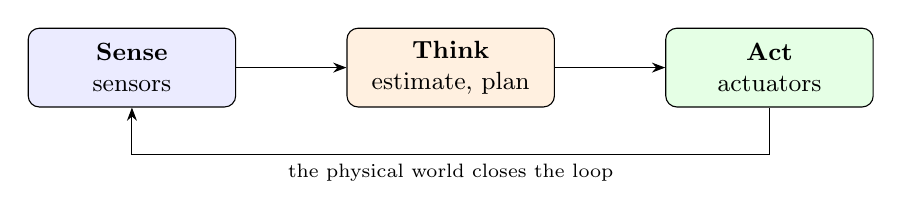
\begin{tikzpicture}[node distance=14mm, every node/.style={font=\small},
			box/.style={draw, rounded corners, minimum height=10mm, text width=24mm, align=center}]
			\node[box, fill=blue!8] (s) {\textbf{Sense}\\sensors};
			\node[box, right=of s, fill=orange!12] (t) {\textbf{Think}\\estimate, plan};
			\node[box, right=of t, fill=green!10] (a) {\textbf{Act}\\actuators};
			\draw[-{Stealth}] (s) -- (t); \draw[-{Stealth}] (t) -- (a);
			\draw[-{Stealth}] (a) -- ++(0,-1.1) -| node[pos=0.25, below, font=\scriptsize] {the physical world closes the loop} (s);
		\end{tikzpicture}
	\end{center}
	\takeaway{A robot is a closed-loop system that \emph{measures} the physical world and \emph{changes} it. Every topic today is one box in this loop.}
\end{frame}

\begin{frame}{Who works on which part of a robot}
	\begin{center}
		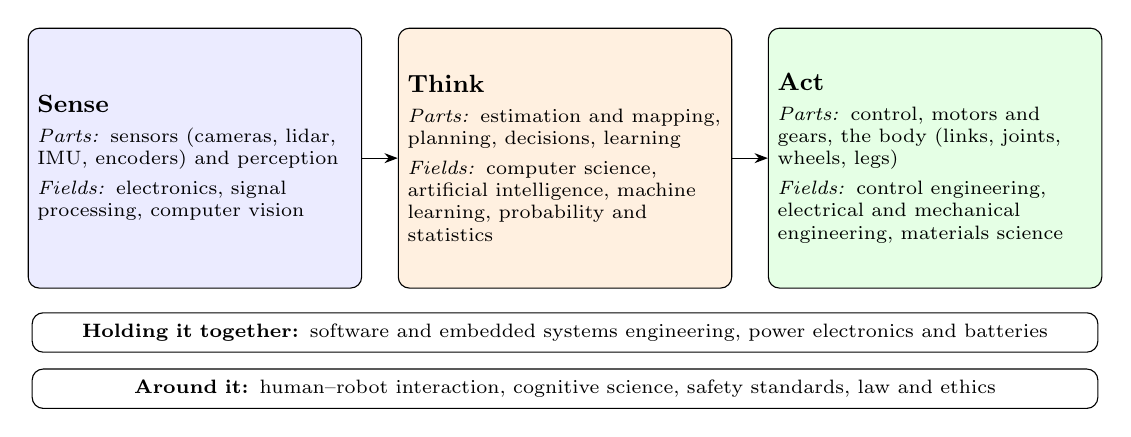
\begin{tikzpicture}[every node/.style={font=\scriptsize},
			col/.style={draw, rounded corners, text width=40mm, minimum height=33mm, align=left, anchor=north, execute at begin node={\hyphenpenalty=10000\exhyphenpenalty=10000}},
			bar/.style={draw, rounded corners, text width=133mm, align=center, minimum height=5mm}]
			\node[col, fill=blue!8] (s) at (0,0) {{\small\textbf{Sense}}\\[1mm]
				\textit{Parts:} sensors (cameras, lidar, IMU, encoders) and perception\\[1mm]
				\textit{Fields:} electronics, signal processing, computer vision};
			\node[col, fill=orange!12] (t) at (47mm,0) {{\small\textbf{Think}}\\[1mm]
				\textit{Parts:} estimation and mapping, planning, decisions, learning\\[1mm]
				\textit{Fields:} computer science, artificial intelligence, machine learning, probability and statistics};
			\node[col, fill=green!10] (a) at (94mm,0) {{\small\textbf{Act}}\\[1mm]
				\textit{Parts:} control, motors and gears, the body (links, joints, wheels, legs)\\[1mm]
				\textit{Fields:} control engineering, electrical and mechanical engineering, materials science};
			\draw[-{Stealth}] (s.east) -- (t.west);
			\draw[-{Stealth}] (t.east) -- (a.west);
			\node[bar, below=3mm of t] (sw) {\textbf{Holding it together:} software and embedded systems engineering, power electronics and batteries};
			\node[bar, below=2mm of sw] {\textbf{Around it:} human--robot interaction, cognitive science, safety standards, law and ethics};
		\end{tikzpicture}
	\end{center}
	\takeaway{No single field builds a robot. Most hard problems in robotics sit where two of these boxes meet.}
\end{frame}

\begin{frame}{Two ways to make a robot move}
	\begin{columns}[T]
		\begin{column}{0.2\textwidth}
			\centering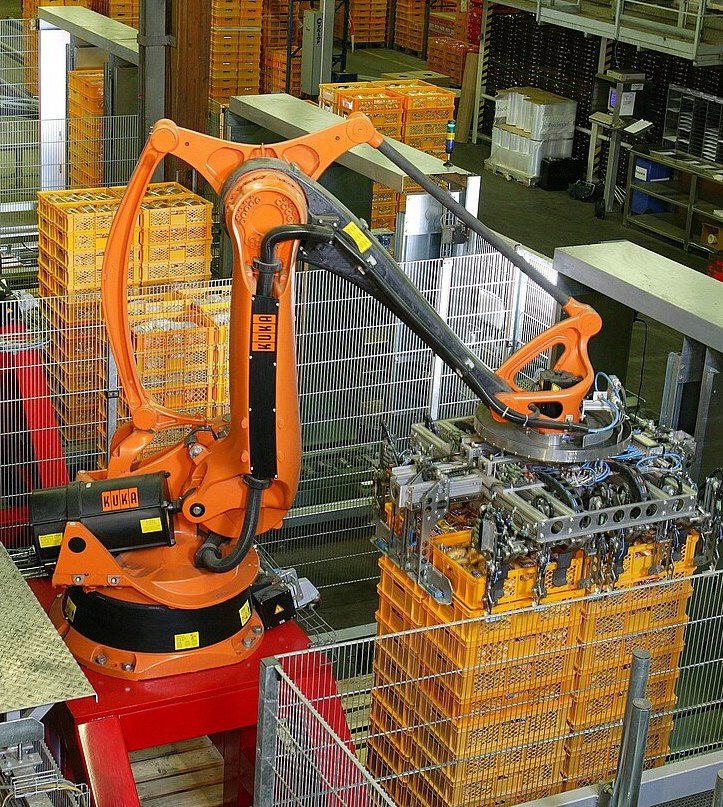
\includegraphics[width=\textwidth]{img/web/factory_kuka_palletizing.jpg}\\[0.5mm]
			{\scriptsize KUKA palletizing cell:\\ the explicit way\par}
		\end{column}
		\begin{column}{0.39\textwidth}
			\begin{block}{Explicit: model the physics}
				\footnotesize
				Engineers describe the robot and the task with models, then compute what to do.\\[1mm]
				Classical control, planning, trajectory optimization.\\[1mm]
				\textbf{Works best} when the physics is well known and the environment is tidy. This is every factory robot today.
			\end{block}
		\end{column}
		\begin{column}{0.37\textwidth}
			\begin{block}{Implicit: learn it from data}
				\footnotesize
				Show the robot examples, or let it try, and let it work out by itself what to do in each situation (a \textbf{policy}).\\[1mm]
				Reinforcement learning, imitation learning.\\[1mm]
				\textbf{Works best} when the world is messy: contact, friction, soft objects, clutter.
			\end{block}
		\end{column}
	\end{columns}
	\vspace{2mm}
	\takeaway{Today we stay on the left. Weeks 4--8 are on the right. Same robots, same problems, different tools.}
\end{frame}

\begin{frame}{Ask: what changes?}
	\begin{center}
		\begin{tabular}{lll}
			\toprule
			\textbf{Mainly the world changes} & \textbf{Manipulation} & arm, gripper, tool use \\
			\textbf{Mainly the robot moves} & \textbf{Locomotion} & wheeled, legged, aerial \\
			\textbf{Both} & \textbf{Mobile manipulation} & mobile base + arm, humanoid \\
			\bottomrule
		\end{tabular}
	\end{center}
	\vspace{4mm}
	\centering \textbf{Try it:} a robot opens a door. What changes?
	\takeaway{This one question tells you what to sense, what the robot can do, and how to measure success.}
\end{frame}

\begin{frame}{Classification by structure}
	\begin{center}
		\begin{tabular}{lll}
			\toprule
			\textbf{Structure} & \textbf{Example} & \textbf{What is easy, what is hard} \\
			\midrule
			Serial chain & UR5, Franka & knowing where the hand is: easy \\
			Parallel & Stewart platform, Delta & the opposite \\
			Tree / branched & humanoid, quadruped & many chains share one body \\
			Wheeled & differential drive, car-like & cannot move sideways \\
			Legged & biped, quadruped (GO2) & contact comes and goes \\
			Aerial & multirotor & never at rest \\
			\bottomrule
		\end{tabular}
	\end{center}
	\takeaway{The mechanical structure decides which problems are cheap. That is why factories standardised on 6-axis arms, and why walking robots took thirty years longer.}
\end{frame}

\begin{frame}{What they look like}
	\centering\scriptsize
	\robotcell{img/web/type_serial_ur16e.jpg}{\textbf{Serial chain}: UR16e arm}\hfill
	\robotcell{img/web/type_parallel_flexpicker.jpg}{\textbf{Parallel}: ABB FlexPicker delta robot}\hfill
	\robotcell{img/web/type_humanoid_atlas.jpg}{\textbf{Tree}: Atlas humanoid}\\[3mm]
	\robotcell{img/web/type_wheeled_turtlebot3.jpg}{\textbf{Wheeled}: TurtleBot3, differential drive}\hfill
	\robotcell{img/web/type_legged_anymal.jpg}{\textbf{Legged}: ANYmal quadruped}\hfill
	\robotcell{img/web/type_aerial_mavic.jpg}{\textbf{Aerial}: quadcopter drone}
\end{frame}

\begin{frame}{Degrees of freedom}
	\begin{itemize}
		\item \textbf{Degree of freedom (DoF)}: one independent way the system can move.
		\item A free object in space has \textbf{6}: move along three axes, rotate about three axes.
		\item A UR5 arm has \textbf{6 joints}: enough to set the tool's position and its orientation together, but not every orientation is possible everywhere. Near the edge of its reach, the choice shrinks.
		\item Ask for the tool \emph{position} only, and 3 joints' worth of freedom is left over: the arm is \textbf{redundant}.
	\end{itemize}
	\takeaway{Redundancy is not waste. It is the freedom to reach the same point while avoiding an obstacle, a joint limit, or an awkward pose.}
\end{frame}

\begin{frame}{Links, joints, frames}
	\begin{columns}[T]
		\begin{column}{0.5\textwidth}
			\begin{itemize}\footnotesize
				\item \textbf{Link}: a rigid piece of the robot.
				\item \textbf{Joint}: the connection that lets two links move relative to each other. Revolute (turns), prismatic (slides), fixed.
				\item \textbf{Frame}: a coordinate system glued to a link. ``Where is this piece, and which way is it facing?''
				\item \textbf{URDF}: the text file that lists all of this, as a \textbf{kinematic tree}: every link except the base has exactly one parent.
			\end{itemize}
		\end{column}
		\begin{column}{0.5\textwidth}
			\centering
			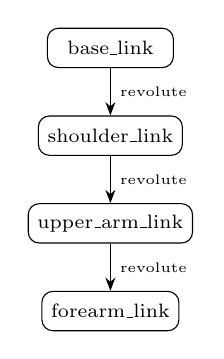
\begin{tikzpicture}[every node/.style={font=\scriptsize}, node distance=6mm,
				l/.style={draw, rounded corners, minimum width=16mm, minimum height=5mm}]
				\node[l] (b) {base\_link};
				\node[l, below=of b] (s) {shoulder\_link};
				\node[l, below=of s] (u) {upper\_arm\_link};
				\node[l, below=of u] (f) {forearm\_link};
				\draw[-{Stealth}] (b) -- node[right, font=\tiny] {revolute} (s);
				\draw[-{Stealth}] (s) -- node[right, font=\tiny] {revolute} (u);
				\draw[-{Stealth}] (u) -- node[right, font=\tiny] {revolute} (f);
			\end{tikzpicture}
		\end{column}
	\end{columns}
	\takeaway{Every number a robot reports (joint angle, sensor reading, detected object) lives in \emph{some} frame. Half of practical robotics is knowing which one.}
\end{frame}

\begin{frame}{Lab tour: classify the real ones}
	\begin{block}{First the tour, then the task}
		We show you around the lab: arm, quadruped, humanoid, mobile base. Then, in groups of two or three, one robot per group: look, touch where allowed, ask.
	\end{block}
	For your robot, write down:
	\begin{enumerate}
		\item how many links and joints you can find, and what kind of joints,
		\item its degrees of freedom, and whether the task usually leaves some over,
		\item the shape of its kinematic tree: one chain, or several branches from one body,
		\item the ``what changes?'' category, and one thing it clearly \emph{cannot} do.
	\end{enumerate}
	\vspace{2mm}
	At the end: one sentence per group.
\end{frame}

\wordsframe{sense--think--act \quad manipulation \quad locomotion \\[3mm] link \quad joint \quad frame \quad URDF \\[3mm] degree of freedom \quad redundancy}

% ===================== 2. WHERE IS THE HAND =====================
\section{Where is the hand?}

\begin{frame}{Two questions every arm must answer}
	\begin{center}
		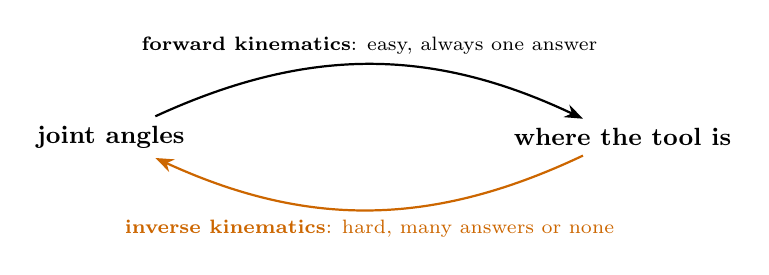
\begin{tikzpicture}[every node/.style={font=\small}]
			\node (q) at (0,0) {\textbf{joint angles}};
			\node (p) at (6.5,0) {\textbf{where the tool is}};
			\draw[-{Stealth}, thick] (q) to[bend left=25] node[above, font=\scriptsize] {\textbf{forward kinematics}: easy, always one answer} (p);
			\draw[-{Stealth}, thick, orange!80!black] (p) to[bend left=25] node[below, font=\scriptsize] {\textbf{inverse kinematics}: hard, many answers or none} (q);
		\end{tikzpicture}
	\end{center}
	\vspace{2mm}
	\begin{itemize}
		\item The motors and encoders only know \textbf{joint angles}.
		\item The task is always given as \textbf{where the tool should be}.
		\item Kinematics is the translation between these two languages.
	\end{itemize}
\end{frame}

\begin{frame}{A pose is a position plus a way of facing}
	\begin{columns}[T]
		\begin{column}{0.52\textwidth}
			\begin{itemize}\footnotesize
				\item \textbf{Position}: where the point is. Three numbers.
				\item \textbf{Orientation}: which way it faces. Three more.
				\item Together: a \textbf{pose}. Six numbers, one rigid object.
				\item A \textbf{rotation} is stored as a small matrix. Its columns are simply the new axes drawn in the old frame. All rotations together are called \textbf{SO(2)} in the plane, \textbf{SO(3)} in space (special orthogonal group).
			\end{itemize}
		\end{column}
		\begin{column}{0.44\textwidth}
			\centering
			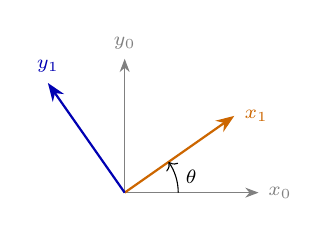
\begin{tikzpicture}[scale=0.85, every node/.style={font=\scriptsize}]
				\draw[-{Stealth}, gray] (0,0) -- (2,0) node[right] {$x_0$};
				\draw[-{Stealth}, gray] (0,0) -- (0,2) node[above] {$y_0$};
				\draw[-{Stealth}, thick, orange!80!black] (0,0) -- (35:2) node[right] {$x_1$};
				\draw[-{Stealth}, thick, blue!70!black] (0,0) -- (125:2) node[above] {$y_1$};
				\draw[->] (0.8,0) arc (0:35:0.8) node[midway, right] {$\theta$};
			\end{tikzpicture}
		\end{column}
	\end{columns}
	\takeaway{A rotation matrix cannot stretch or squash anything. That is the mathematical way of saying ``rigid body''. And undoing a rotation costs nothing.}
\end{frame}

\begin{frame}{A frame is a point of view}
	\begin{itemize}
		\item The same object has different coordinates in different frames. Nothing moved, only the observer.
		\item A \textbf{transform} is the recipe to move a measurement from one frame to another: a rotation and a shift, packed together.
		\item Robots pack rotation and shift into one matrix (the \textbf{homogeneous transform}) so that changing frames is a single multiplication. All poses together are called \textbf{SE(2)} in the plane, \textbf{SE(3)} in space (special Euclidean group). Notebook 1 uses these names.
	\end{itemize}
	\vspace{2mm}
	\centering \footnotesize \texttt{T\_base\_camera}: where the camera is, seen from the base. The same matrix turns a point measured by the camera into base coordinates.
	\takeaway{In most robot code, read \texttt{T\_A\_B} as ``B, as seen from A'', but check each library's convention. Getting this backwards is one of the most common bugs in robotics.}
\end{frame}

\begin{frame}{The arm is a chain of frames}
	\begin{center}
		\begin{minipage}[c]{0.4\textwidth}\centering
		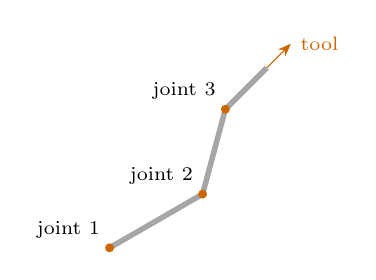
\begin{tikzpicture}[scale=0.62, every node/.style={font=\scriptsize}]
			\coordinate (o) at (0,0);
			\coordinate (a) at (30:2.2);
			\coordinate (b) at ($(a)+(75:1.8)$);
			\coordinate (c) at ($(b)+(45:1.2)$);
			\draw[line width=2pt, gray!70] (o) -- (a) -- (b) -- (c);
			\foreach \p/\n in {o/{joint 1}, a/{joint 2}, b/{joint 3}} {
				\fill[orange!80!black] (\p) circle (2.6pt);
				\node[above left] at (\p) {\n};
			}
			\draw[-{Stealth}, orange!80!black] (c) -- ++(45:0.7) node[right] {tool};
		\end{tikzpicture}
		\end{minipage}\hfill
		\begin{minipage}[c]{0.56\textwidth}\centering
			\animategraphics[autoplay,loop,width=0.95\textwidth,poster=24]{12}{img/sim/order_matters_frames/f-}{0}{47}\\[0.3mm]
			{\tiny\href{https://raw.githubusercontent.com/ABC-iRobotics/advanced-robotics-project-course/main/week01_classical_robotics/slides/img/sim/order_matters.gif}{\textcolor{blue!70!black}{play in the browser}}}
		\end{minipage}
	\end{center}
	\begin{itemize}\footnotesize
		\item Walk from the base outwards: at each joint, ``turn by this angle, then go along the link in the turned direction''.
		\item Multiplying these steps, from the base outwards, gives the tool pose. That is all forward kinematics is.
		\item \textbf{Order matters}: turn-then-go is not go-then-turn. Try it with your hand. Right: the same arm simulated both ways.
	\end{itemize}
	\takeaway{Forward kinematics: walk along the arm, one turn-then-go step per joint.}
\end{frame}

\begin{frame}{Denavit--Hartenberg (DH) parameters}
	\begin{columns}[T]
		\begin{column}{0.52\textwidth}
			\begin{itemize}\footnotesize
				\item In 3D, getting from one joint frame to the next takes 6 numbers in general. The DH convention places the frames so that \textbf{4 per joint} are enough:
				\item $\theta$, \textbf{joint angle}: turn about the joint axis $z$. This is the number that changes when the joint moves.
				\item $d$, \textbf{offset} along that $z$; then $a$, \textbf{link length} along the new $x$.
				\item $\alpha$, \textbf{twist} about that $x$, lining $z$ up with the next joint axis.
				\item Careful: datasheets use \emph{standard} or \emph{modified} DH.
			\end{itemize}
		\end{column}
		\begin{column}{0.44\textwidth}
			\centering\scriptsize
			\textbf{UR5, standard DH}\\[1mm]
			\begin{tabular}{crrrr}
				\toprule
				joint & $\theta$ & $d$ [m] & $a$ [m] & $\alpha$ \\
				\midrule
				1 & $q_1$ & 0.089 & 0 & $90^\circ$ \\
				2 & $q_2$ & 0 & $-0.425$ & $0^\circ$ \\
				3 & $q_3$ & 0 & $-0.392$ & $0^\circ$ \\
				4 & $q_4$ & 0.109 & 0 & $90^\circ$ \\
				5 & $q_5$ & 0.095 & 0 & $-90^\circ$ \\
				6 & $q_6$ & 0.082 & 0 & $0^\circ$ \\
				\bottomrule
			\end{tabular}\\[1mm]
			rounded to mm; Notebook 1, Part C uses this table
		\end{column}
	\end{columns}
	\takeaway{Four numbers per joint, one row per joint: the whole arm fits in a small table. Each row is one ``turn, then go'' step, now in 3D.}
\end{frame}

\begin{frame}{Inverse kinematics: three things to expect}
	\begin{columns}[T]
		\begin{column}{0.52\textwidth}
			\begin{enumerate}\footnotesize
				\item \textbf{Several answers.} Elbow-up and elbow-down reach the same point. A 6-axis arm typically has eight. The controller has to \emph{choose}.
				\item \textbf{No answer.} Outside the \textbf{workspace} there is nothing to compute. Reach has a boundary.
				\item \textbf{Sometimes no formula.} A \emph{closed-form solution} is a direct formula, like the one for the two-link arm in Notebook 1. Arm makers often design their arms so that one exists (the UR5 has one). For a general arm there is none, and the answer is found numerically, by nudging.
			\end{enumerate}
		\end{column}
		\begin{column}{0.46\textwidth}
			\centering
			\animategraphics[autoplay,loop,width=\textwidth,poster=10]{15}{img/sim/ik_answers_frames/f-}{0}{59}\\[0.3mm]
			{\tiny\href{https://raw.githubusercontent.com/ABC-iRobotics/advanced-robotics-project-course/main/week01_classical_robotics/slides/img/sim/ik_answers.gif}{\textcolor{blue!70!black}{play in the browser}}}
		\end{column}
	\end{columns}
\end{frame}

\begin{frame}{The Jacobian: which way does the tool go?}
	\begin{itemize}
		\item Move \emph{one} joint a tiny bit. The tool moves a tiny bit in some direction.
		\item The \textbf{Jacobian} is the table of those directions, one column per joint.
		\item With it you can ask: ``I want the tool to go \emph{there}, how should the joints move?''
		\item In some poses, no combination of joint moves can push the tool in a certain direction: that direction is missing from the table. Such a pose is a \textbf{singularity}.
	\end{itemize}
	\takeaway{Stretch your arm out fully and try to move your hand further away. You cannot. Your elbow is at a singularity.}
\end{frame}

\begin{frame}{Solving IK by nudging}
	\begin{columns}[T]
		\begin{column}{0.52\textwidth}
			\begin{enumerate}\footnotesize
				\item Look where the tool is now. Measure the gap to the target.
				\item Use the Jacobian to turn that gap into a small joint move.
				\item Take the step. Repeat until the gap is tiny.
			\end{enumerate}
			\vspace{2mm}
			\footnotesize
			The \textbf{solver} is this whole loop. The \textbf{pseudo-inverse} is the tool used in step 2: it turns the gap into a joint move, and when many joint moves would do, it picks the \textbf{smallest} one.\\[2mm]
			Run the same loop once per control cycle, and the solver \emph{is} the controller.
		\end{column}
		\begin{column}{0.44\textwidth}
			\centering
			\animategraphics[autoplay,loop,height=5.2cm,poster=last,trim=121 81 125 67]{6}{img/UR5animation/UR5_pinv--}{1}{36}\\[0.5mm]
			{\tiny the solver, one frame per step \quad \href{https://raw.githubusercontent.com/ABC-iRobotics/advanced-robotics-project-course/main/week01_classical_robotics/slides/img/sim/ur5_ik_solver.gif}{\textcolor{blue!70!black}{play in the browser}}}
		\end{column}
	\end{columns}
\end{frame}

\begin{frame}{Notebook 1: build it yourself}
	\begin{block}{Open in Colab, 30 minutes}
		\texttt{Notebook 1 -- Forward and Inverse Kinematics}\\ {\scriptsize \href{https://colab.research.google.com/github/ABC-iRobotics/advanced-robotics-project-course/blob/main/week01_classical_robotics/notebooks/nb1_fk_ik_STUDENT.ipynb}{\textcolor{blue!70!black}{Open in Colab}}, or find it at \href{https://github.com/ABC-iRobotics/advanced-robotics-project-course}{\textcolor{blue!70!black}{github.com/ABC-iRobotics/advanced-robotics-project-course}}}
	\end{block}
	\begin{itemize}
		\item \textbf{A}: frames and transforms, forward kinematics of a planar arm, with sliders.
		\item \textbf{B}: inverse kinematics of a two-link arm, both elbows, the workspace boundary.
		\item \textbf{C}: a real UR5 in 3D, the Jacobian, IK by nudging, then closing the loop. \emph{We run this one together and watch.}
	\end{itemize}
	\vspace{2mm}
	This is where the matrices live. A and B have four one-line exercises, each followed by a check cell that tells you whether it is right. We fill them in together.
\end{frame}

\wordsframe{pose \quad frame \quad transform \quad DH parameters \\[3mm] forward kinematics \quad inverse kinematics \quad workspace \\[3mm] Jacobian \quad singularity \quad pseudo-inverse}

% ===================== 3. SENSING =====================
\section{How a robot sees}

\begin{frame}{What a robot can measure}
	\begin{center}
		\begin{tabular}{lll}
			\toprule
			& \textbf{About itself} & \textbf{About the world} \\
			& \emph{proprioceptive} & \emph{exteroceptive} \\
			\midrule
			Examples & joint encoders, IMU, & camera, depth camera, \\
			         & joint torque sensors & lidar, tactile, GPS \\
			Speed & very fast & slower \\
			Character & precise, but \emph{drifts} when integrated & noisy, but \emph{anchored to the world} \\
			\bottomrule
		\end{tabular}
	\end{center}
	\takeaway{The two families fail in opposite ways. That is exactly why robots combine them: this is called \textbf{sensor fusion}.}
\end{frame}

\begin{frame}{The IMU and why you cannot navigate with it}
	\begin{itemize}
		\item An \textbf{IMU} measures how fast the robot is \emph{accelerating} and \emph{turning}. Not where it is.
		\item \textbf{Velocity} is how fast position changes; \textbf{acceleration} is how fast velocity changes. Going back means adding up over time (\textbf{integrating}): acceleration gives velocity, velocity gives position. Two sums in a row, so a tiny constant error grows with time squared.
		\item After a few seconds of ``IMU only'', the position estimate is fiction.
	\end{itemize}
	\begin{center}
		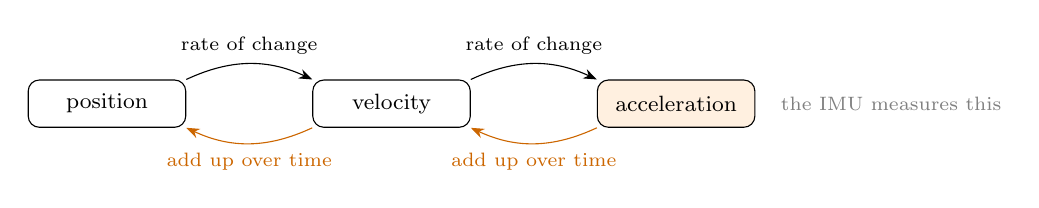
\begin{tikzpicture}[node distance=16mm, every node/.style={font=\footnotesize},
			b/.style={draw, rounded corners, minimum height=6mm, minimum width=20mm}]
			\node[b] (p) {position};
			\node[b, right=of p] (v) {velocity};
			\node[b, right=of v, fill=orange!12] (a) {acceleration};
			\node[right=2mm of a, font=\scriptsize, text=gray] {the IMU measures this};
			\draw[-{Stealth}] (p.north east) to[bend left=25] node[above, font=\scriptsize] {rate of change} (v.north west);
			\draw[-{Stealth}] (v.north east) to[bend left=25] node[above, font=\scriptsize] {rate of change} (a.north west);
			\draw[-{Stealth}, orange!80!black] (a.south west) to[bend left=25] node[below, font=\scriptsize] {add up over time} (v.south east);
			\draw[-{Stealth}, orange!80!black] (v.south west) to[bend left=25] node[below, font=\scriptsize] {add up over time} (p.south east);
		\end{tikzpicture}
	\end{center}
	{\scriptsize Video: \href{https://youtu.be/_q_8d0E3tDk?t=130}{\textcolor{blue!70!black}{Pure IMU-based positional tracking is a no-go}} (Oliver Kreylos, 5\,min). The position estimate floats away from 2:15.\par}
	\takeaway{Something has to look at the world and pull the drifting estimate back: a lidar, a camera, a GPS. Sensor fusion is not optional.}
\end{frame}

\begin{frame}{Lidar and depth cameras: geometry from light}
	\begin{itemize}
		\item Lidar and time-of-flight cameras: send light out, time how long it takes to come back, get a distance, thousands of times per second. Stereo and structured-light depth cameras triangulate instead, from two views or a projected pattern.
		\item The result is a \textbf{point cloud}: a cloud of 3D points, \emph{as seen from the sensor}.
		\item To use it, the robot has to move the points into its own frame. That is the transform from the previous section.
	\end{itemize}
	\takeaway{A sensor never tells you where the wall is. It tells you where the wall is \emph{relative to the sensor}. The frames do the rest.}
\end{frame}

\begin{frame}{Seeing with a camera}
	\begin{center}
		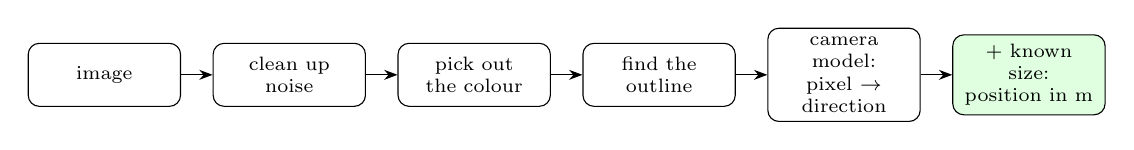
\begin{tikzpicture}[node distance=4mm, every node/.style={font=\scriptsize},
			b/.style={draw, rounded corners, minimum height=8mm, text width=17mm, align=center}]
			\node[b] (i) {image};
			\node[b, right=of i] (f) {clean up\\noise};
			\node[b, right=of f] (s) {pick out\\the colour};
			\node[b, right=of s] (c) {find the\\outline};
			\node[b, right=of c] (k) {camera model:\\pixel $\to$ direction};
			\node[b, right=of k, fill=green!12] (p) {+ known size:\\position in m};
			\foreach \a/\b in {i/f, f/s, s/c, c/k, k/p} \draw[-{Stealth}] (\a) -- (\b);
		\end{tikzpicture}
	\end{center}
	\vspace{2mm}
	\begin{itemize}\footnotesize
		\item \textbf{Clean up noise}: classical image filters, for example a Gaussian or a median filter, blur away single wrong pixels. \textbf{Camera model}: turns a pixel into a direction from the camera; a known object size then gives the distance.
		\item Every step is a hand-written rule. Works brilliantly under factory lighting, falls apart when the world changes.
	\end{itemize}
	\takeaway{One camera gives you a \emph{direction}, not a distance. Depth needs a second view, a depth sensor, or a known object size.}
\end{frame}

\begin{frame}{Where am I? Localization, mapping, SLAM}
	\begin{center}
		\begin{tabular}{ll}
			\toprule
			\textbf{Localization} & the map is known, find the robot on it \\
			\textbf{Mapping} & the robot's path is known, draw the map \\
			\textbf{SLAM} & neither is known: do both at the same time \\
			\bottomrule
		\end{tabular}
	\end{center}
	\vspace{3mm}
	\begin{itemize}\footnotesize
		\item While driving, the uncertainty about ``where am I'' \textbf{grows}.
		\item Seeing a known landmark makes it \textbf{shrink}.
		\item Recognising a place you have visited before is a \textbf{loop closure}: the accumulated error snaps back.
	\end{itemize}
	\vspace{1mm}{\scriptsize Video: \href{https://youtu.be/A0H8CoORZJU?t=205}{\textcolor{blue!70!black}{LIO-SAM lidar mapping}} (Tixiao Shan, 9\,min). Doubled walls from drift at 3:40, then ``A loop is closed.'' at 3:45.\par}
	\takeaway{SLAM is a chicken-and-egg problem. It is solved by demanding that all measurements agree with each other at once.}
\end{frame}

\wordsframe{proprioceptive \quad exteroceptive \quad sensor fusion \\[3mm] IMU \quad drift \quad point cloud \quad depth \\[3mm] localization \quad mapping \quad SLAM \quad loop closure}

% ===================== 4. MOBILE ROBOT =====================
\section{How a robot drives}

\begin{frame}{The differential drive}
	\begin{columns}[T]
		\begin{column}{0.52\textwidth}
			\begin{itemize}\footnotesize
				\item Two driven wheels, one on each side. Same speed: straight. Different speeds: it turns.
				\item The robot's \textbf{state}: where it is and which way it faces, $(x, y, \theta)$.
				\item What we command: forward speed $v$ and turning rate $\omega$.
				\item It \textbf{cannot move sideways}. Robots with this limitation are called \textbf{nonholonomic}.
			\end{itemize}
		\end{column}
		\begin{column}{0.44\textwidth}
			\centering
			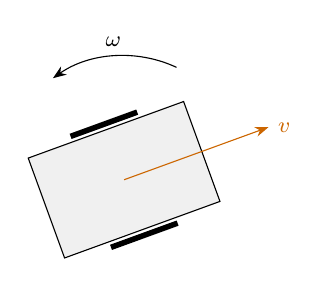
\begin{tikzpicture}[scale=1.5, every node/.style={font=\footnotesize}]
				\draw[rotate=20, fill=gray!12] (-0.7,-0.45) rectangle (0.7,0.45);
				\draw[rotate=20, line width=2pt] (-0.3,-0.5) -- (0.3,-0.5);
				\draw[rotate=20, line width=2pt] (-0.3,0.5) -- (0.3,0.5);
				\draw[-{Stealth}, orange!80!black] (0,0) -- (20:1.3) node[right] {$v$};
				\draw[-{Stealth}] (65:1.05) arc (65:125:1.05) node[midway, above] {$\omega$};
			\end{tikzpicture}
		\end{column}
	\end{columns}
	\takeaway{It can reach any pose, just not directly. Parallel parking is the everyday proof.}
\end{frame}

\begin{frame}{Go-to-goal: the smallest useful controller}
	\begin{columns}[c]
		\begin{column}{0.54\textwidth}
			\begin{itemize}\footnotesize
				\item Two things the robot can measure: \textbf{how far} the goal is (the \textbf{distance error} $\rho$), and \textbf{how far off} its heading is (the \textbf{heading error} $\alpha$).
				\item Two rules: drive faster when the goal is far, turn harder when the heading is off.
				\item That is \textbf{proportional feedback}: the correction is proportional to the error.
			\end{itemize}
		\end{column}
		\begin{column}{0.42\textwidth}
			\centering
			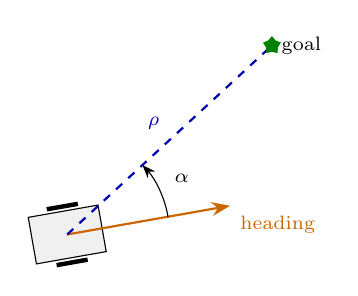
\begin{tikzpicture}[scale=1.0, every node/.style={font=\scriptsize}]
				\coordinate (r) at (0,0); \coordinate (g) at (2.6,2.4);
				\draw[rotate=10, fill=gray!12] (-0.45,-0.3) rectangle (0.45,0.3);
				\draw[rotate=10, line width=1.6pt] (-0.2,-0.36) -- (0.2,-0.36);
				\draw[rotate=10, line width=1.6pt] (-0.2,0.36) -- (0.2,0.36);
				\draw[-{Stealth}, thick, orange!80!black] (r) -- (10:2.1) node[below right] {heading};
				\draw[dashed, thick, blue!70!black] (r) -- node[above left] {$\rho$} (g);
				\node[star, star points=5, fill=green!50!black, inner sep=1.6pt] at (g) {};
				\node[right] at (g) {goal};
				\draw[-{Stealth}] (10:1.3) arc (10:42.7:1.3);
				\node at (26:1.62) {$\alpha$};
			\end{tikzpicture}
		\end{column}
	\end{columns}
	\vspace{2mm}
	\footnotesize One classic bug: if the heading error is not wrapped to $\pm 180^\circ$, the robot turns the long way round.
	\takeaway{Feedback means: measure the error, push against it, repeat. The arm controller in Notebook 1 did exactly the same thing.}
\end{frame}

\begin{frame}{Planning: which way around the shelf?}
	\begin{itemize}
		\item Cut the floor into a grid of cells: free or blocked. Grow the blocked cells by the robot's size, so the robot can be treated as a point.
		\item \textbf{A*} searches the grid for the cheapest path, guided by a guess of the remaining distance.
		\item The output is a list of \textbf{waypoints}. No speeds, no timing.
		\item Other planners you will meet: Dijkstra, D* Lite (fast replanning), Theta* (any-angle paths), Hybrid A* (car-like robots), and the sampling-based PRM, RRT and RRT*.
	\end{itemize}
	\takeaway{The planner answers a geometric question (which way), the controller answers a dynamic one (how fast). Keeping them separate is what makes the classical stack manageable.}
\end{frame}

\begin{frame}{Sequencing: the finite state machine}
	\begin{center}
		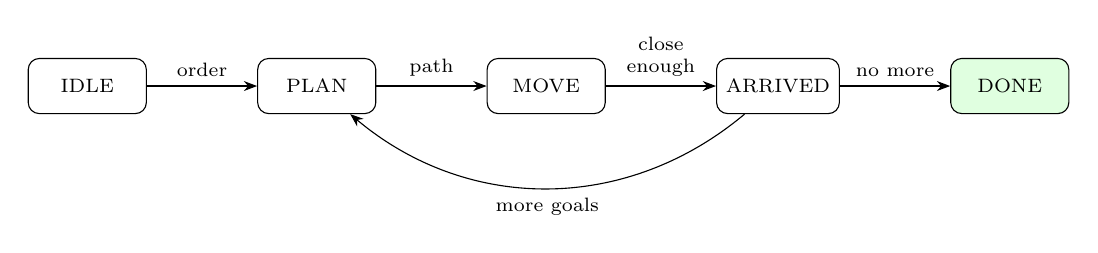
\begin{tikzpicture}[node distance=14mm, every node/.style={font=\scriptsize},
			s/.style={draw, rounded corners, minimum height=7mm, minimum width=15mm}]
			\node[s] (i) {IDLE};
			\node[s, right=of i] (p) {PLAN};
			\node[s, right=of p] (m) {MOVE};
			\node[s, right=of m] (a) {ARRIVED};
			\node[s, right=of a, fill=green!12] (d) {DONE};
			\draw[-{Stealth}] (i) -- node[above, font=\scriptsize] {order} (p);
			\draw[-{Stealth}] (p) -- node[above, font=\scriptsize] {path} (m);
			\draw[-{Stealth}] (m) -- node[above, font=\scriptsize, align=center] {close\\enough} (a);
			\draw[-{Stealth}] (a) -- node[above, font=\scriptsize] {no more} (d);
			\draw[-{Stealth}] (a) to[bend left=40] node[below, font=\scriptsize] {more goals} (p);
		\end{tikzpicture}
	\end{center}
	\takeaway{Behaviour is a sequence of modes. Inside each mode, the continuous controller runs. This is how industrial robots have been programmed for forty years.}
\end{frame}

\begin{frame}{Notebook 2: drive a robot around a warehouse}
	\begin{block}{Open in Colab, 25 minutes}
		\texttt{Notebook 2 -- Mobile Robot Navigation}\\ {\scriptsize \href{https://colab.research.google.com/github/ABC-iRobotics/advanced-robotics-project-course/blob/main/week01_classical_robotics/notebooks/nb2_mobile_robot_STUDENT.ipynb}{\textcolor{blue!70!black}{Open in Colab}}, or find it at \href{https://github.com/ABC-iRobotics/advanced-robotics-project-course}{\textcolor{blue!70!black}{github.com/ABC-iRobotics/advanced-robotics-project-course}}}
	\end{block}
	\begin{itemize}
		\item A differential-drive robot you can steer.
		\item The go-to-goal controller.
		\item A warehouse grid map and A* path planning.
		\item A state machine that visits a list of goals, animated end to end.
	\end{itemize}
	Four short exercises, each followed by a check cell. The animation you produce here is the same kind you will hand in with H1.
\end{frame}

\wordsframe{differential drive \quad nonholonomic \quad state \\[3mm] feedback \quad proportional control \\[3mm] path planning \quad A* \quad waypoint \quad state machine}

% ===================== 5. BEYOND =====================
\section{Building behaviour}

\begin{frame}{Manipulation, locomotion, whole-body control}
	\begin{itemize}
		\item \textbf{Manipulation}: plan a path for the tool, turn it into joint motion with IK, follow it.
		\item \textbf{Locomotion}: decide where the feet go and when they touch the ground.
		\item \textbf{Whole-body control}: move \emph{all} joints at once so that balance, contact and the task are satisfied together, hundreds of times per second.
	\end{itemize}
	\takeaway{A legged robot is an arm that manipulates the ground. The difference is that it has to let go at every step, and still not fall.}
\end{frame}

\begin{frame}{From state machines to behaviour trees}
	\begin{columns}[T]
		\begin{column}{0.47\textwidth}
			\centering \textbf{State machine}\\[1mm]
			\footnotesize Every new situation adds arrows everywhere. ``What if the battery runs low?'' needs an arrow out of every state.
		\end{column}
		\begin{column}{0.47\textwidth}
			\centering \textbf{Behaviour tree}\\[1mm]
			\footnotesize A tree of small tasks, checked from the top many times a second. Each task reports success, failure, or still running.
		\end{column}
	\end{columns}
	\vspace{3mm}
	\begin{itemize}\footnotesize
		\item \textbf{Sequence}: do these in order. \textbf{Fallback}: try these until one works. \textbf{Retry}: try again.
		\item A recovery behaviour is one fallback branch, added in one place.
		\item Nav2, the ROS 2 navigation stack, uses a behaviour tree to decide when to plan, drive and recover.
	\end{itemize}
	\takeaway{Same behaviour, better organised. This is an engineering answer, not a mathematical one.}
\end{frame}

\begin{frame}{End-to-end: skipping the pipeline}
	\begin{center}
		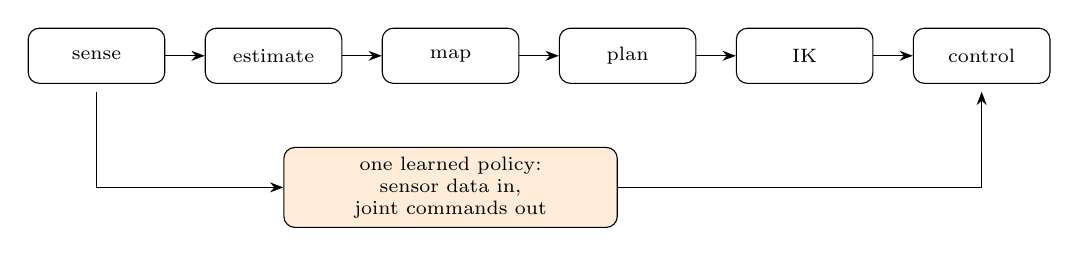
\begin{tikzpicture}[node distance=5mm, every node/.style={font=\scriptsize},
			b/.style={draw, rounded corners, minimum height=7mm, text width=15mm, align=center}]
			\node[b] (s) {sense};
			\node[b, right=of s] (e) {estimate};
			\node[b, right=of e] (m) {map};
			\node[b, right=of m] (p) {plan};
			\node[b, right=of p] (k) {IK};
			\node[b, right=of k] (c) {control};
			\foreach \a/\b in {s/e, e/m, m/p, p/k, k/c} \draw[-{Stealth}] (\a) -- (\b);
			\node[b, below=8mm of m, fill=orange!15, text width=40mm] (nn) {one learned policy:\\sensor data in, joint commands out};
			\draw[-{Stealth}] ($(s.south)+(0,-0.1)$) |- (nn.west);
			\draw[-{Stealth}] (nn.east) -| ($(c.south)+(0,-0.1)$);
		\end{tikzpicture}
	\end{center}
	\footnotesize \textbf{Policy}: the rule that decides what the robot does next, given what it senses. A \emph{learned} policy is found from data instead of written by hand.\par
	\textbf{Why people try this:} the hand-built boxes are brittle where they meet, they choke on raw camera, touch and sound data, contact and soft objects resist modelling, and there is more and more robot data to learn from.
	\takeaway{This is the bridge to weeks 4--8. The learned policy still sends its commands to the same joints. Keep today's vocabulary.}
\end{frame}

\wordsframe{whole-body control \\[3mm] state machine \quad behaviour tree \quad sequence \quad fallback \\[3mm] end-to-end \quad policy}

% ===================== 6. INDUSTRY =====================
\section{Industry landscape}

\begin{frame}{The numbers, 2024}\small
	\begin{center}
		\begin{tabular}{ll}
			\toprule
			Industrial robots installed worldwide & 542\,076 robots \\
			Share by region & Asia 74\,\%, Europe 16\,\%, Americas 9\,\% \\
			China's share of these & 54\,\% (295\,000 robots) \\
			Chinese vendors' share of their home market & 57\,\% (about 28\,\% a decade ago) \\
			Robots in operation worldwide (the ``stock'') & 4\,664\,000 robots \\
			Robots in operation in China & over 2\,000\,000, five times the US \\
			Installed in Europe & 85\,000 robots, 8\,\% fewer than in 2023 \\
			Installed in Germany & 26\,982 robots, 5\,\% fewer than in 2023 \\
			\bottomrule
		\end{tabular}
	\end{center}
	\vspace{2mm}
	\footnotesize Industrial robots only; one unit is one robot. ``Installed'' means put into service during 2024. Source: IFR World Robotics 2025, ifr.org.
\end{frame}

\begin{frame}{Europe: the legacy and the new wave}
	\begin{columns}[T]
		\begin{column}{0.46\textwidth}
			\textbf{Established}
			\begin{itemize}\footnotesize
				\item KUKA (DE), ABB (CH/SE)
				\item Universal Robots (DK): the collaborative arm as a product category
				\item Germany is still the largest European market
			\end{itemize}
		\end{column}
		\begin{column}{0.5\textwidth}
			\textbf{New wave}
			\begin{itemize}\footnotesize
				\item ANYbotics (ETH spin-off): legged inspection
				\item Agile Robots (DE): force-controlled manipulation
				\item Neura Robotics (DE): cognitive robots, humanoids
			\end{itemize}
		\end{column}
	\end{columns}
	\takeaway{Europe's strength has been precision, safety and integration. The open question is whether that carries into the learning-driven generation.}
\end{frame}

\begin{frame}{China and the United States}
	\begin{columns}[T]
		\begin{column}{0.47\textwidth}
			\textbf{China}
			\begin{itemize}\footnotesize
				\item Volume, vertical integration, aggressive pricing
				\item Unitree, UBTech and others put quadrupeds and humanoids within a university budget
				\item The GO2 in our lab exists because of this
			\end{itemize}
		\end{column}
		\begin{column}{0.47\textwidth}
			\textbf{United States}
			\begin{itemize}\footnotesize
				\item Boston Dynamics, Figure, Tesla Optimus
				\item Strength in software, foundation models and capital
			\end{itemize}
		\end{column}
	\end{columns}
	\vspace{3mm}
	\centering \textbf{Question for you:} where does Europe fit, and what would it take to change that?
\end{frame}

\begin{frame}{Where the field is going}
	\begin{center}
		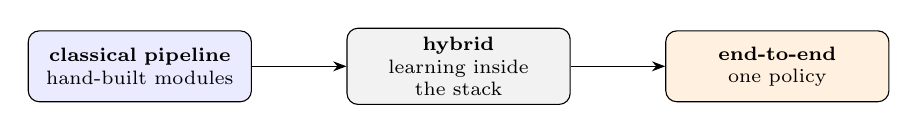
\begin{tikzpicture}[node distance=12mm, every node/.style={font=\scriptsize},
			b/.style={draw, rounded corners, minimum height=9mm, text width=26mm, align=center}]
			\node[b, fill=blue!8] (a) {\textbf{classical pipeline}\\hand-built modules};
			\node[b, right=of a, fill=gray!10] (b) {\textbf{hybrid}\\learning inside\\the stack};
			\node[b, right=of b, fill=orange!12] (c) {\textbf{end-to-end}\\one policy};
			\draw[-{Stealth}] (a) -- (b); \draw[-{Stealth}] (b) -- (c);
		\end{tikzpicture}
	\end{center}
	\vspace{3mm}
	\begin{itemize}
		\item The classical tools do not disappear. They run \emph{inside} modern systems: IK, controllers, planners, state estimators.
		\item That is why we spent today on them.
	\end{itemize}
\end{frame}

% ===================== 7. HOMEWORK =====================
\section{Homework}

\begin{frame}{H1: warehouse AMR}
	\begin{block}{Scenario}
		An autonomous mobile robot serves a warehouse. It receives an order: a list of shelves to visit in a given sequence, then it delivers to the packing station.
	\end{block}
	\textbf{You get:} a template notebook with a new warehouse map, the order, the A* planner, the path follower and the video export.\\
	\textbf{You write:} the state machine for the full cycle, plus \emph{one} realistic complication of your choice:
	\begin{enumerate}\footnotesize
		\item battery level, with a detour to the charging station,
		\item a blocked aisle discovered on the way, requiring replanning,
		\item several orders, sequenced by travel distance.
	\end{enumerate}
	\textbf{Submit:} the notebook, the generated animation as a video, and a one-page description. \textbf{Deadline: week 4, 2 October.}
\end{frame}

\begin{frame}{Next week}
	\begin{block}{Literature research and scientific methods}
		How to find, read, filter and cite work in robotics, and how to turn a vague interest into a researchable question.
	\end{block}
	\vspace{3mm}
	Bring one topic you would like to work on. We will search it together, in class.\par
	\vspace{5mm}
	\centering \footnotesize Slides and notebooks: Moodle and \href{https://github.com/ABC-iRobotics/advanced-robotics-project-course}{\textcolor{blue!70!black}{github.com/ABC-iRobotics/advanced-robotics-project-course}}. Questions: after class or by email.
\end{frame}

\thankyouforattentionframe{}

% ===================== BACKUP =====================
\section{Backup}

\begin{frame}{Backup slides}
	\centering Shown only if there is time, or on request.
\end{frame}

\begin{frame}{Demo: real sensor data, replayed}
	\begin{block}{3 minutes, in the browser, nothing installed}
		A real self-driving car recording (nuScenes) in the Rerun viewer: lidar, radars, six cameras and the car's pose, all on one timeline.\\[1mm]
		{\scriptsize \href{https://app.rerun.io/version/0.37.1/?url=https://app.rerun.io/version/0.37.1/examples/nuscenes_dataset.rrd}{\textcolor{blue!70!black}{app.rerun.io: nuScenes example}}\par}
	\end{block}
	Watch for:
	\begin{itemize}
		\item the boxes sit on the cars in the camera images only because every frame and transform is right,
		\item the sensors arrive at completely different rates: lidar 20 times a second, cameras 12, labels 2,
		\item no drift here: the car's pose was already corrected against a prebuilt map. Raw odometry would drift.
	\end{itemize}
\end{frame}

\begin{frame}{Live: a humanoid in the browser}
	\begin{block}{Demo, 2 minutes}
		A physics simulator (MuJoCo) and a trained policy, both running inside one browser tab: a Unitree G1 humanoid following motions.\\[1mm]
		{\scriptsize \href{https://motion-tracking.axell.top/}{\textcolor{blue!70!black}{motion-tracking.axell.top}} \quad backup: \href{https://php-parkour.github.io/demo.html}{\textcolor{blue!70!black}{php-parkour.github.io/demo.html}}\par}
	\end{block}
	\begin{itemize}
		\item MuJoCo is a physics engine many research labs train in.
		\item The policy outputs joint targets, exactly where our IK output went.
		\item Drag the robot with the mouse: it recovers, because the policy keeps correcting.
		\item Nothing was installed. Your project demos can look like this.
	\end{itemize}
\end{frame}

\begin{frame}{Grasping, the classical view}
	\begin{columns}[T]
		\begin{column}{0.55\textwidth}
			\begin{itemize}\footnotesize
				\item Two fingers, two contact points, facing each other: an \textbf{antipodal grasp}.
				\item Each finger can only push within a cone set by friction. Outside it, the object slips.
				\item If the fingers can resist any push or twist, the grasp has \textbf{force closure}. It will hold.
			\end{itemize}
		\end{column}
		\begin{column}{0.42\textwidth}
			\centering
			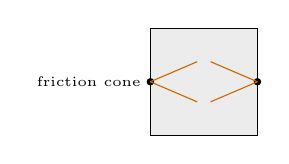
\begin{tikzpicture}[scale=0.85, every node/.style={font=\tiny}]
				\draw[fill=gray!15] (0,0) rectangle (1.6,1.6);
				\fill (0,0.8) circle (1.6pt); \fill (1.6,0.8) circle (1.6pt);
				\draw[orange!80!black] (0,0.8) -- (0.7,1.1); \draw[orange!80!black] (0,0.8) -- (0.7,0.5);
				\draw[orange!80!black] (1.6,0.8) -- (0.9,1.1); \draw[orange!80!black] (1.6,0.8) -- (0.9,0.5);
				\node[left] at (0,0.8) {friction cone};
			\end{tikzpicture}
		\end{column}
	\end{columns}
	\takeaway{Classical grasping needs the object's shape and its friction. In real life you know neither. That is why modern grasping is learned from images.}
\end{frame}

\begin{frame}{Fleet management}
	\begin{itemize}
		\item One robot becomes a \emph{system}: who does which task, who yields in the corridor, who charges when, robots from different vendors in one hall.
		\item The question is no longer ``which joint angle'' but ``which robot, in which order''.
		\item Success is measured in orders per hour, not millimetres.
	\end{itemize}
	\takeaway{At this level the robot is a resource. The hard problems become scheduling, but a bad low-level controller still ruins the whole schedule.}
\end{frame}

% ===================== SOURCES =====================
\begin{frame}{Sources: videos, demos, definitions}
	\scriptsize
	\textbf{Videos}
	\begin{itemize}
		\item IMU drift: Oliver Kreylos, ``Pure IMU-based Positional Tracking is a No-go'', \url{https://youtu.be/_q_8d0E3tDk}
		\item Loop closure: Tixiao Shan, ``LIO-SAM: Tightly-coupled Lidar Inertial Odometry via Smoothing and Mapping'', \url{https://youtu.be/A0H8CoORZJU}
	\end{itemize}
	\textbf{Demos}
	\begin{itemize}
		\item Recorded sensor data: Rerun web viewer, nuScenes example, \url{https://app.rerun.io/}
		\item Humanoid in the browser: \url{https://motion-tracking.axell.top/}, backup \url{https://php-parkour.github.io/demo.html}
	\end{itemize}
	\textbf{Definitions and numbers}
	\begin{itemize}
		\item Robot definition: ISO 8373:2021 Robotics -- Vocabulary, term 3.1, \url{https://www.iso.org/standard/75539.html}
		\item Industry numbers: IFR World Robotics 2025, \url{https://ifr.org/}
	\end{itemize}
\end{frame}

\begin{frame}{Image credits}
	\scriptsize All photos are from Wikimedia Commons and used under the licence given.
	\begin{itemize}\scriptsize
		\item Industrial robots on a car body line (slide 2): Steve Jurvetson, \href{https://creativecommons.org/licenses/by/2.0/}{CC BY 2.0}, cropped.\\ \url{https://commons.wikimedia.org/wiki/File:Tesla_Robot_Dance_(7408451314).jpg}
		\item KUKA robots palletizing bread (slide 11): KUKA Roboter GmbH, Bachmann, public domain, cropped.\\ \url{https://commons.wikimedia.org/wiki/File:Factory_Automation_Robotics_Palettizing_Bread.jpg}
		\item UR16e robot arm (slide 14): Auledas, \href{https://creativecommons.org/licenses/by-sa/4.0/}{CC BY-SA 4.0}.\\ \url{https://commons.wikimedia.org/wiki/File:UR16e_robot_arm.png}
		\item ABB FlexPicker delta robot (slide 14): Marc Auledas, \href{https://creativecommons.org/licenses/by-sa/4.0/}{CC BY-SA 4.0}.\\ \url{https://commons.wikimedia.org/wiki/File:Robot_delta_FlexPicker_d'ABB.png}
		\item Atlas humanoid, 2013 (slide 14): DARPA, public domain.\\ \url{https://commons.wikimedia.org/wiki/File:Atlas_frontview_2013.jpg}
		\item TurtleBot3 Burger (slide 14): Kuscu0, \href{https://creativecommons.org/licenses/by-sa/4.0/}{CC BY-SA 4.0}.\\ \url{https://commons.wikimedia.org/wiki/File:TurtleBot3_Burger.jpg}
		\item ANYmal quadruped (slide 14): ANYbotics, \href{https://creativecommons.org/licenses/by-sa/4.0/}{CC BY-SA 4.0}.\\ \url{https://commons.wikimedia.org/wiki/File:ANYbotics_robot_dog_ANYmal.jpg}
		\item DJI Mavic Air 2 quadcopter (slide 14): C.Stadler/Bwag, \href{https://creativecommons.org/licenses/by-sa/4.0/}{CC BY-SA 4.0}.\\ \url{https://commons.wikimedia.org/wiki/File:DJI_-_Drohne_Mavic_Air_2.JPG}
	\end{itemize}
\end{frame}

\end{document}
